\documentclass{beamer}

% ----- Latex properties
\usepackage[latin1]{inputenc}
\usepackage{tikz} % 2D drawing
\usepackage{graphicx} % enhanced graphics
\graphicspath{ {img/} }

% ----- Beamer theme properties
\usetheme[left,hideothersubsections]{Goettingen}
\usecolortheme{crane,sidebartab}
\usefonttheme{structureitalicserif}
\useinnertheme[shadow]{rounded}
\setbeamercovered{transparent}

\theoremstyle{definition}
\newtheorem{researchquestion}[theorem]{Research question}



% ----- Document properties
\title[Statistical Properties of DKD]
{%
Investigating the Statistical Properties\\
of the Double Kernel Density Estimator
}
\author[Harold Ship]
{%
    Harold~Ship
    \\
    {%
    \small
    Advisors: Prof.~Boris~Portnov \and
    Dr.~Itai~Dattner \and
    Prof.~Em.~Benjamin~Reiser
    }
}
\institute[University~of~Haifa]
{%
University~of~Haifa \and 
Faculty~of~Management \and
Department~of~Information~\&~Knowledge~Management
}

\date{January 30, 2019}

%
% ----- The presentation
%
\begin{document}

% ----- Title page
\begin{frame}
\tikz [remember picture,overlay]
    \node at
        ([xshift=0.9cm, yshift=-3.6cm]current page.west) 
        {
\includegraphics[width=1.5cm]{univ_logo2.png}};
    \titlepage
\end{frame}

% ----- SECTION: Introduction
\section*{Introduction}

\begin{frame}\frametitle{Mapping disease incidence}
    \begin{center}{ 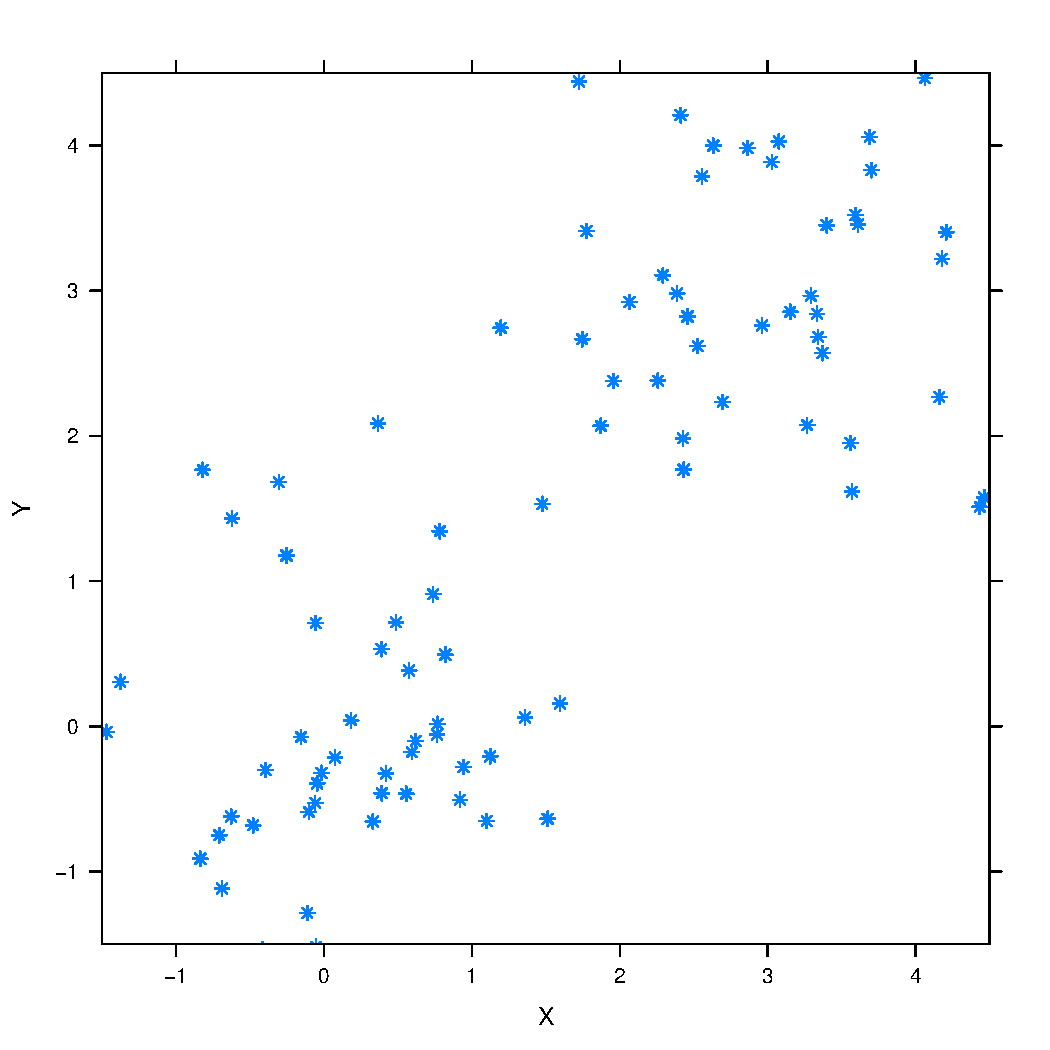
\includegraphics[width=0.5\textwidth]{example-incidents} }\end{center}
    \begin{itemize}
        \item Is there a pattern here?
        \item Does it simply reflect population density?
        \item Or is the risk of disease higher in some locations?
    \end{itemize}
\end{frame}

\begin{frame}\frametitle{The double kernel density}
    \begin{itemize}
        \item The \emph{double kernel density} (DKD) has been used in the literature \cite{kloog2009using}, \cite{portnov2009studying}, \cite{zusman2012residential}
        \item The statistical properties of the DKD have not been studied
        \item This research:
        \begin{itemize}
            \item Looks to build a methodological framework for studying some of the statistical properties
            \item Methodology will be based on computer simulations of the stochastic process of disease incidence
            \item Will assess the performance of the DKD method
        \end{itemize}
    \end{itemize}
\end{frame}

% ----- Outline
\begin{frame}{Outline}
\tableofcontents[hideallsubsections]
\end{frame}

% ----- SECTION: Theoretical background
\section{Theoretical background}

% ----- SUBSECTION: Measuring disease risk
\subsection{Measuring disease risk}
\begin{frame}\frametitle{Measuring disease risk}
    \begin{itemize}
        \item How do I measure the risk of developing a disease?
        \item How do I compare the problem of disease in different times and places?
    \end{itemize}
    \begin{definition}
        \alert{Cumulative incidence} or \alert{risk} is the proportion of the at-risk population that develop a disease during the study period.
        \begin{equation*}
            \lambda = \frac{number~of~new~cases~of~disease}{number~of~people~who~can~get~it}
        \end{equation*}
        \cite{bonita2006basic}
    \end{definition}
    \begin{itemize}
        \item We are interested in comparing the risk at different \emph{locations}, represented by $(x,y)$ coordinates
    \end{itemize}
\end{frame}

% ----- SUBSECTION: Smoothing disease cases
\subsection{Smoothing disease cases}
\begin{frame}\frametitle{Smoothing disease cases}
    \begin{itemize}
        \item Are cases of disease concentrated in specific areas?
        \item Administrative boundaries: problematic
            \begin{itemize}
                \item Arbitrary boundaries
                \item Heterogenous populations
                \item Small number of cases: privacy
            \end{itemize}
        \item \alert{Kernel smoothing} to compute \emph{intensity} a.k.a \emph{density}
        \item Accuracy is highly dependent on the \emph{bandwidth} \textbf{(h)} which controls the amount of smoothing
    \end{itemize}
    \begin{example}{\tiny{\textbf{Left:} case locations, smoothed with \textbf{Middle:} small value of \emph{h}. \textbf{Right:} large value of \emph{h}.}}
    \centerline{
        \label{fig:points-and-dkd}
        \centering
        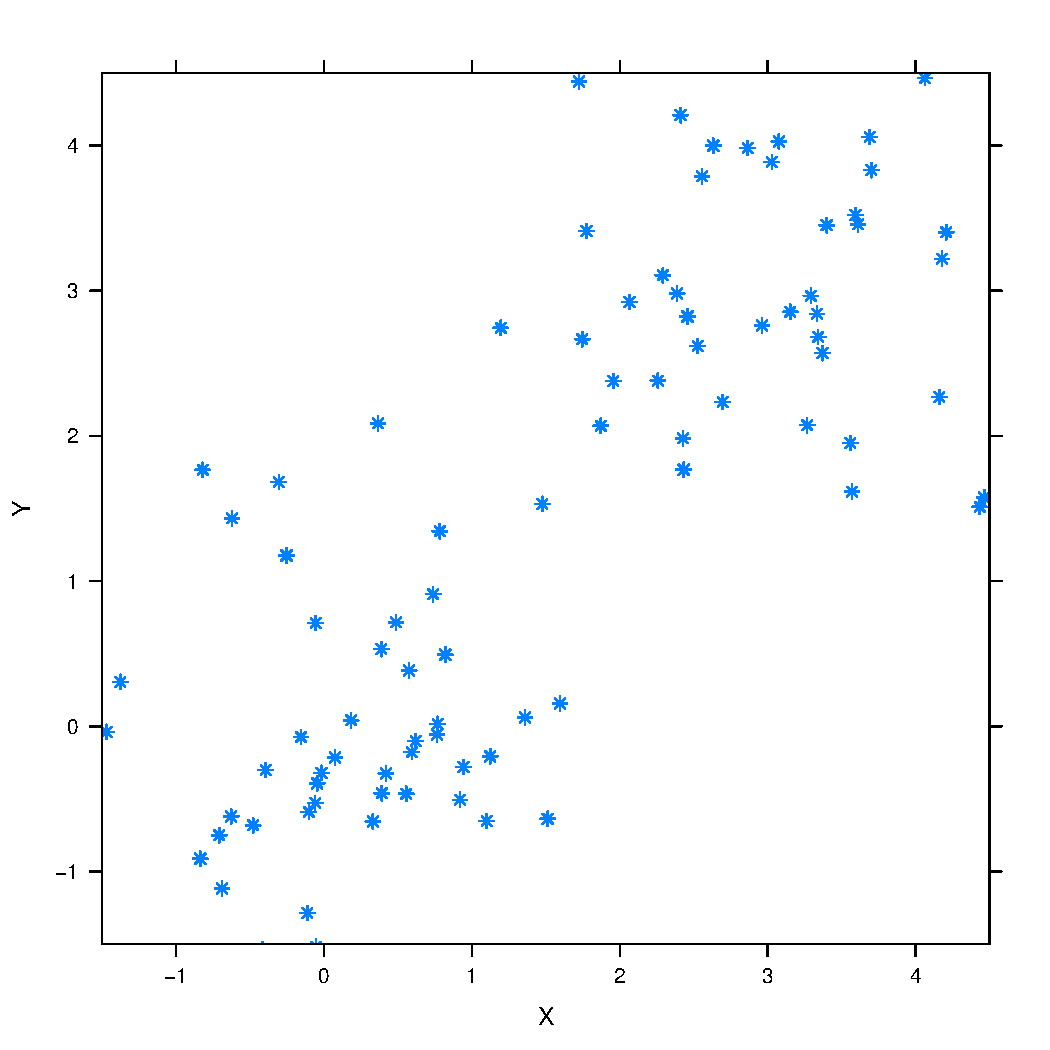
\includegraphics[width=0.3\textwidth]{example-incidents}
        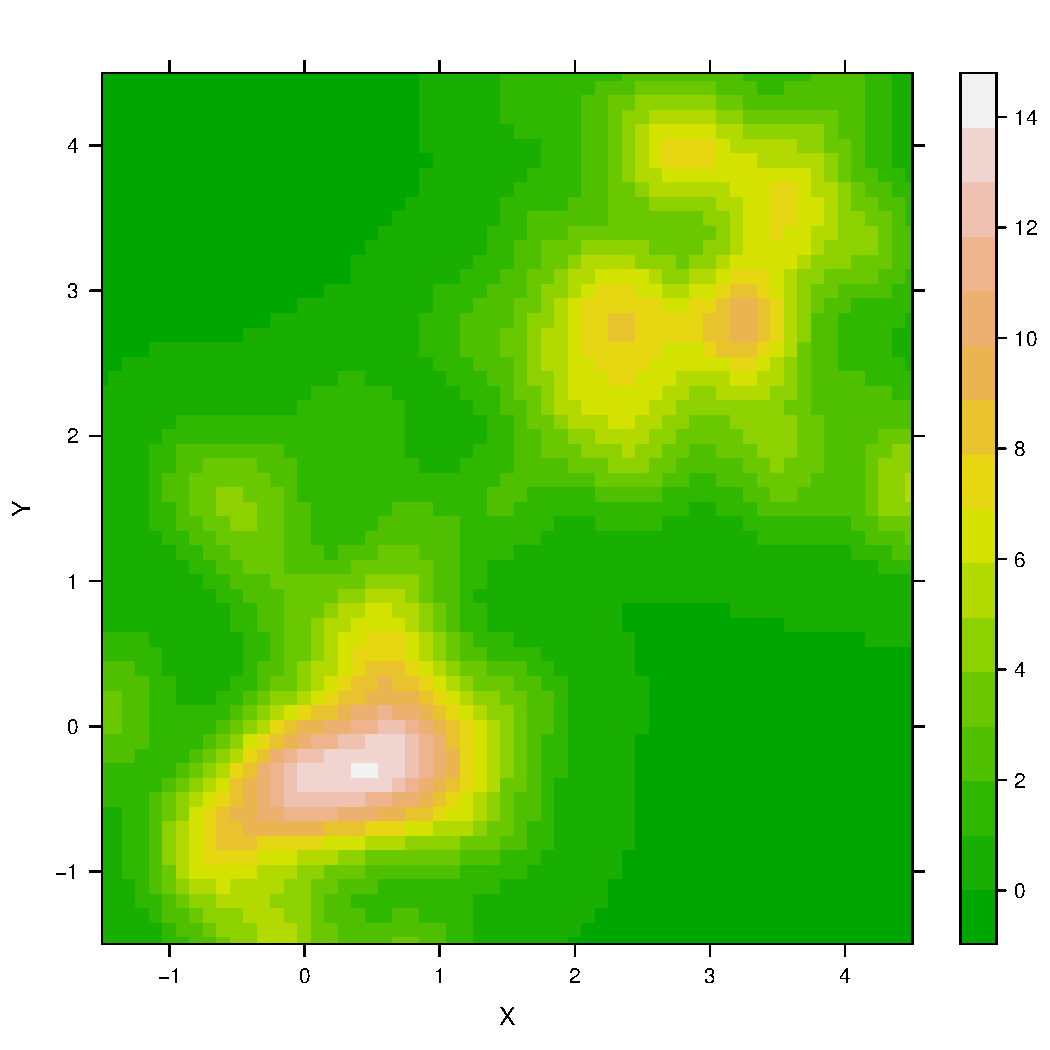
\includegraphics[width=0.3\textwidth]{example-incidents-undersmoothed}
        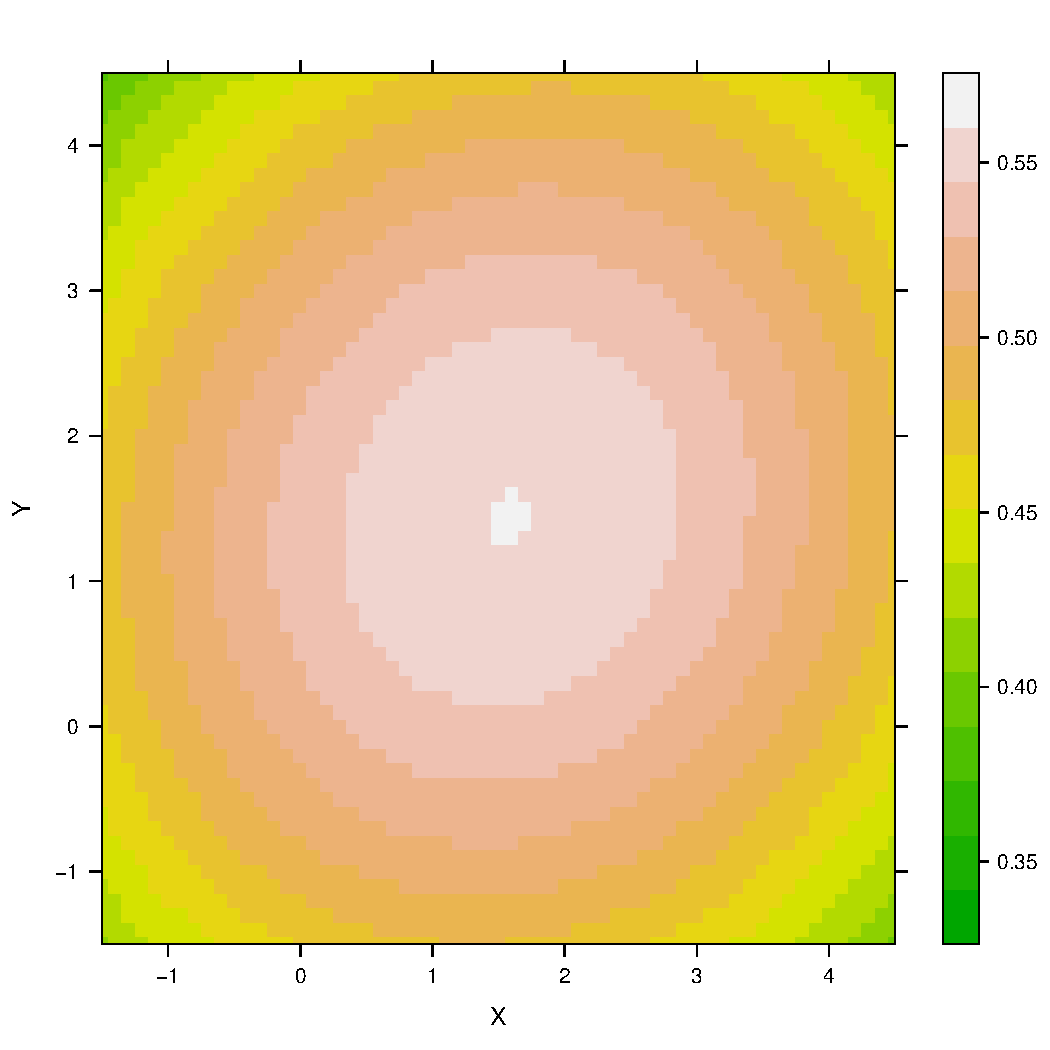
\includegraphics[width=0.3\textwidth]{example-incidents-oversmoothed}
    }
    \end{example}
\end{frame}

% ----- SUBSECTION: Estimating disease risk with the double kernel density
\subsection{Estimating disease risk with the double kernel density}
\begin{frame}\frametitle{Estimating disease risk with the double kernel density}
    \begin{itemize}
        \item We want to know $\lambda$, the risk of developing disease, at a point $(x,y)$
        \item Smooth the cases and the population separately
        \item Divide to get a function \textbf{$\hat{\lambda}$} that \emph{estimates} the risk at any point
    \end{itemize}
    \begin{definition}
        The \alert{double kernel density} estimator is computed at a point by dividing the \emph{disease case intensity} by the \emph{population intensity} at that point.
        \begin{equation*}
            \hat{\lambda}_{dkd}(x,y;h) = \frac{ \hat{\lambda}_{c}(x,y;h) } { \hat{\lambda}_{p}(x,y;h) }
        \end{equation*}
    \end{definition}
\end{frame}

% ----- SUBSECTION: Assessing the performance of the DKD
\subsection{Assessing the performance of the DKD}
\begin{frame}\frametitle{Assessing the performance of the DKD}
    \begin{itemize}
        \item Can we infer the \emph{risk} function from the data?
        \item If so, how ``good'' a job will the DKD do?
        \item Measures of estimation error: mean squared error, mean absolute error, maximum absolute error
        \item Peak location -- Euclidean distance, relative error of the height
    \end{itemize}
\end{frame}

% ----- SECTION: Research questions
\section{Research questions}

\begin{frame}\frametitle{Research questions}
    \begin{researchquestion}[Accuracy of DKD]
        Under what conditions can the DKD be used to accurately estimate the true risk function, taking into account a variety of experimental setups?
    \end{researchquestion}
    \begin{researchquestion}[Magnitude and location of peaks]
        How does the DKD perform in determining the magnitude and location of the peak of the true risk function?
    \end{researchquestion}
\end{frame}

% ----- SECTION: Methodology
\section{Methodology}

\begin{frame}\frametitle{Monte Carlo simulations of DKD}
    \begin{itemize}
        \item Start with the ``truth''
        \item Stochastic model based on Poisson process
        \item Simulation: generate a random sample of points (cases)
        \item Compute the DKD from the sample
        \item Compare it to the ``truth''
        \item Repeat \textellipsis
        \item Then compute the different measures of error
    \end{itemize}
\end{frame}

% ----- SECTION: Preliminary results
\section{Preliminary results}

% ----- SUBSECTION: Results of the error analysis
\subsection{Preliminary results of the error analysis}
\begin{frame}\frametitle{Preliminary results of the error analysis}
    \begin{itemize}
        \item Comparison of measurements of error for different bandwidths:
        \begin{itemize}
            \item a \textbf{small} bandwidth of 20\% of the study area diameter
            \item a \textbf{large} bandwidth of 40\% of the study area diameter
        \end{itemize}
        \item Mean absolute error (MAE), mean squared error (MSE) and maximum absolute error (Sup)
    \end{itemize}
    \begin{table}{Measure of estimation error}
        \centering
        \fbox{%
        \begin{tabular}{l r r}
            Measure & Small Bandwidth & Large Bandwidth \\ \hline
            MAE & 0.0018 & 0.0010 \\
            MSE & 0.0036 & 0.0020 \\
            Sup & 0.0250 & 0.0118
        \end{tabular}
        }% fbox
    \end{table}
\end{frame}

% ----- SUBSECTION: Results of the magnitude of the peaks
\subsection{Preliminary results of the magnitude of the peaks}
\begin{frame}\frametitle{Preliminary results of the magnitude of the peaks}
    \footnotesize
    \begin{itemize}
        \item True value of the peak: 0.248
        \item Bias of peak value: -0.0224 or -9\% (small bandwidth) and -0.0839 or -34\% (large bandwidth)
        \item Standard deviation: 0.0173 or 7\% (small bandwidth) and 0.00841 or 3.4\% (large bandwidth)
        \item 90\% had peak value \alert{less than} the truth (small bandwidth)
        \item 100\% had peak value \alert{less than} the truth (large bandwidth)
    \end{itemize}
    \begin{example}{\tiny{\textbf{Left:} small bandwidth. \textbf{Right:} large bandwidth. \\
    {\color{red}Red} line is true value of $\lambda$ at the peak. {\color{blue}Blue dashed} line is mean.}}
    \centerline{
        \label{fig:peaks-values-hist}
        \centering
        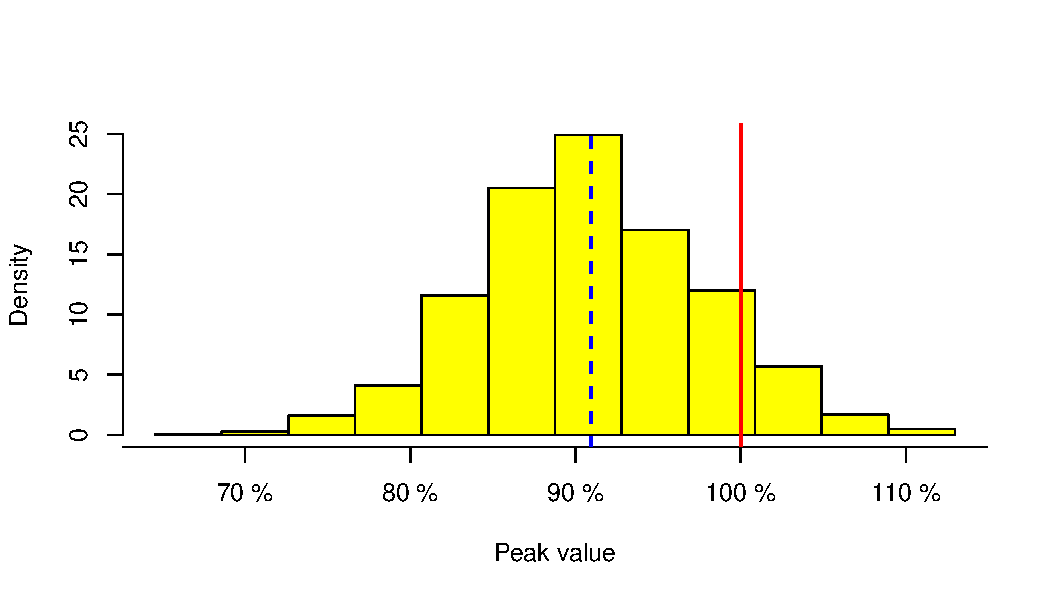
\includegraphics[width=0.5\textwidth]{peaks-hist-values-undersmooth}
        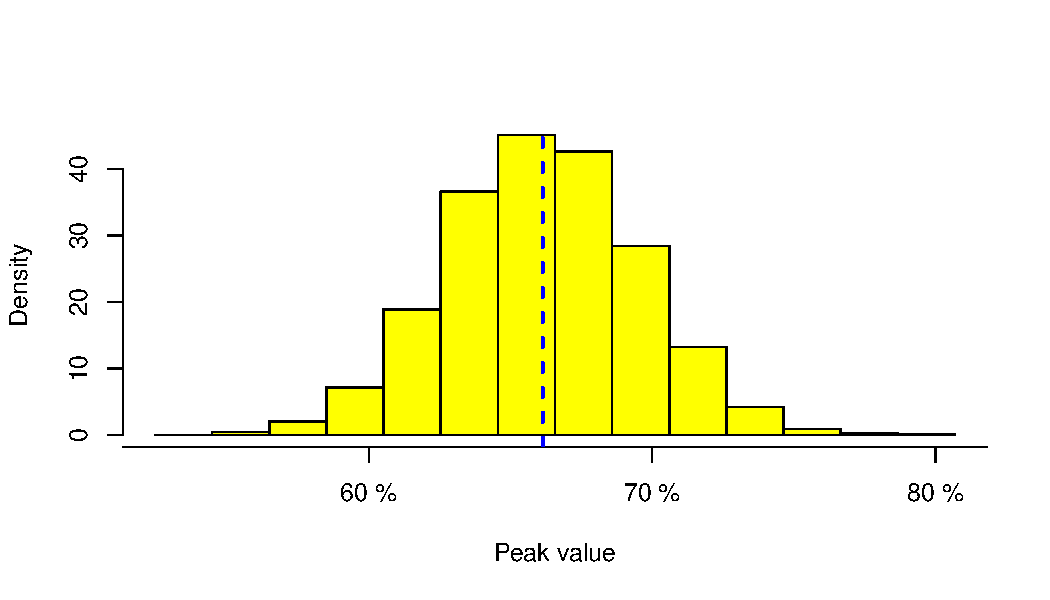
\includegraphics[width=0.5\textwidth]{peaks-hist-values-oversmooth}
     }
    \end{example}
\end{frame}

% ----- SUBSECTION: Results of the location of the peaks
\subsection{Results of the location of the peaks}
\begin{frame}\frametitle{Results of the location of the peaks}
    \footnotesize
    \begin{itemize}
        \item Average displacement of the peak: 0.833, or 3.5\% of study area diameter (small bandwidth) and 0.296 or 1.2\% (large bandwidth)
        \item Standard deviation: 0.466 or 2\% of study area diameter (small bandwidth) and 0.280 or 1.2\% (large bandwidth)
        \item 56\% of the simulations within 0.833 of the truth with the small bandwidth
        \item 46\% of the simulations within 0.296 of the truth with the large bandwidth
    \end{itemize}
    \begin{example}{\tiny{\textbf{Left:} small bandwidth. \textbf{Right:} large bandwidth. {\color{blue}Blue dashed} line is mean.}}
    \centerline{
        \label{fig:peaks-loations-hist}
        \centering
        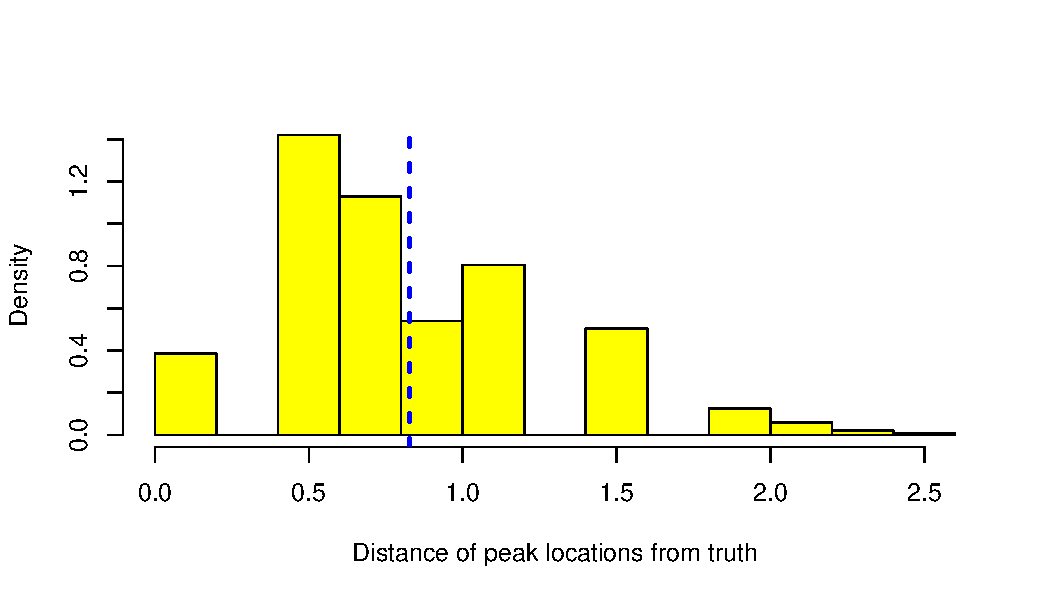
\includegraphics[width=0.5\textwidth]{peaks-hist-locations-undersmooth}
        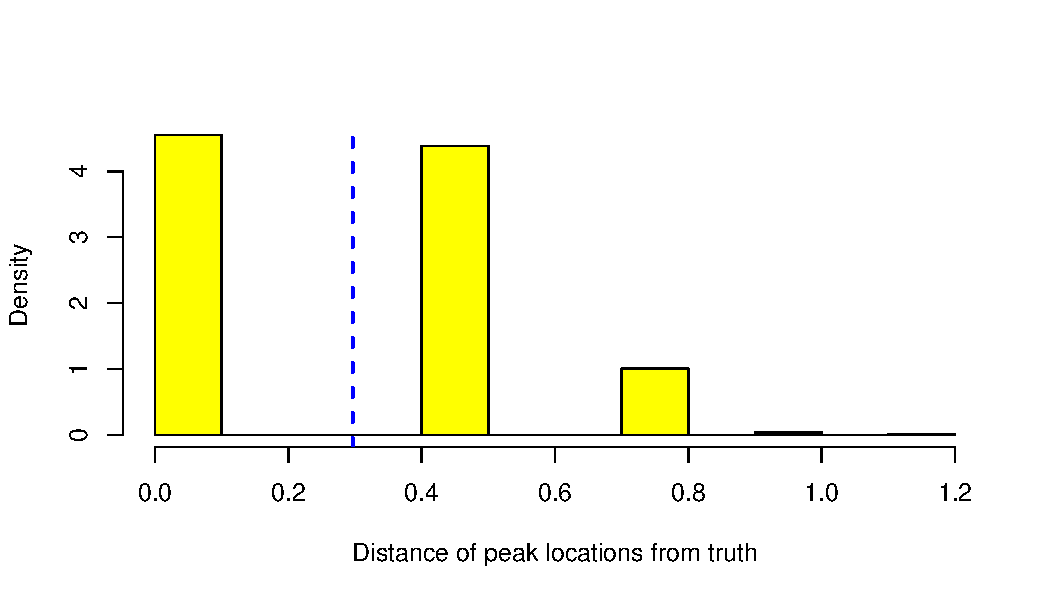
\includegraphics[width=0.5\textwidth]{peaks-hist-locations-oversmooth}
     }
    \end{example}
\end{frame}

% ----- SUBSECTION: Single peak illustration
\subsection{Single peak illustration}
\begin{frame}\frametitle{Single peak illustration}
    \begin{itemize}
        \item Peak location and height can vary
        \item DKD accuracy depends on bandwidth
    \end{itemize}
    \begin{example}{\tiny{\textbf{Left:} small value of $h$. \textbf{Right:} large value of $h$. {\color{red}*} estimated peak. \tikz\draw[blue,fill=blue] (0,0) circle (.5ex); true peak.}}
    \centerline{
        \label{fig:example-peaks}
        \centering
        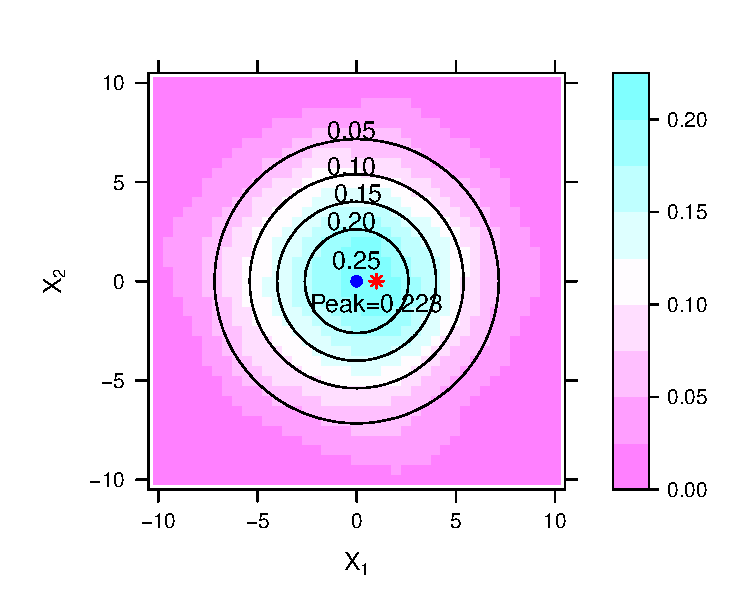
\includegraphics[width=0.5\textwidth]{example-peaks-undersmooth}
        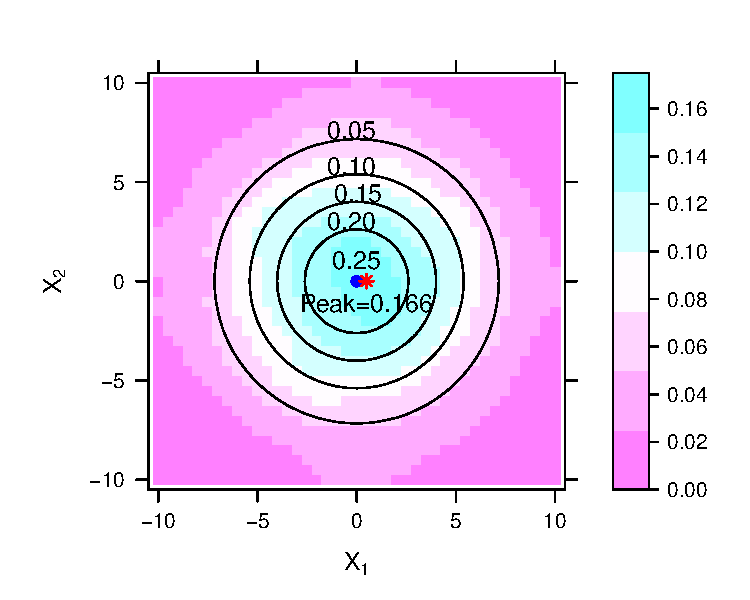
\includegraphics[width=0.5\textwidth]{example-peaks-oversmooth}
     }
    \end{example}
\end{frame}

% ----- SECTION: Discussion
\section{Discussion}

% ----- SUBSECTION: Discussion of the research so far
\subsection{Discussion of the research so far}
\begin{frame}\frametitle{Discussion of the research so far}
    \footnotesize
    \begin{itemize}
        \item Calibrated our ``measuring device'' using a simple setup with uniform population and a single peak of incidents
        \item The present simulation experiment estimates DKD accuracy in terms of magnitude of the true peaks:
        \begin{itemize}
            \scriptsize
            \item within a 9\% error margin and in 90\% of cases underestimates the peak magnitude for the small bandwidth
            \item within a 34\% error margin and in 100\% of cases underestimates the peak magnitude for the large bandwidth
        \end{itemize}
        \item The present simulation experiment estimates DKD accuracy in terms of location of the true peaks:
        \begin{itemize}
            \scriptsize
            \item are within a 3.5\% error margin for 56\% of cases with the small bandwidth
            \item are within a 1.2\% error margin for 46\% of cases with the large bandwidth
        \end{itemize}
        \item Now we would like to:
        \begin{itemize}
            \scriptsize
            \item Derive and evaluate the optimal bandwidth, which minimizes estimation error
            \item Apply our measuring device to realistic scenarios
        \end{itemize}
    \end{itemize}
\end{frame}

% ----- SUBSECTION: Next steps
\subsection{Next steps}
\begin{frame}\frametitle{Next steps}
    In order to complete this research, we plan to do the following:
    \begin{itemize}
        \item Derive the \alert{optimal bandwidth} analytically
        \item \textellipsis and develop a method to estimate it accurately
        \item Vary the number of incidents: use 200, 500, and 1,000
        \item Vary the number of peaks: 1, 2, 3
        \item Use different levels of ``concentration'' of the peak by varying the standard deviation of the ``truth'': 2, 4, 8
        \item Use a non-uniform population, one that also has a peak in the center of the study area
        \item Compute the centroid of the top 5\% of the DKD values instead of the global maximum
    \end{itemize}
\end{frame}

% ----- SECTION: Learning experience
\section{Things I learned doing this research}

\begin{frame}\frametitle{Things I learned doing this research}
    \begin{itemize}
        \item I learned a few things about chronic disease epidemiology
        \begin{itemize}
            \item Incidence versus prevalance
            \item Risk
        \end{itemize}
        \item I mostly learned a lot of statistics
        \begin{itemize}
            \item Unsupervised learning -- density estimation
            \item Measures of error
            \item The importance of sample size
            \item Non-parametric statistics
            \item Monte Carlo simulations
            \item Bootstrap
        \end{itemize}
    \end{itemize}
\end{frame}

% ----- SECTION: References
\section*{References}

\begin{frame}\frametitle{References}
    \footnotesize
    \begin{thebibliography}{10}
        \bibitem[Bonita,~R., Beaglehole,~R., \& Kjellstr{\" o}m,~T., 2006]{bonita2006basic}
            Bonita,~R., Beaglehole,~R., \& Kjellstr{\" o}m,~T.
            Basic epidemiology.
            {\em World Health Organization}, 2006.
        \bibitem[Kloog, I., Haim, A., \& Portnov, B. A., 2009]{kloog2009using}
            Kloog, I., Haim, A., \& Portnov, B. A.
            Using kernel density function as an urban analysis tool: Investigating the association between nightlight exposure and the incidence of breast cancer in Haifa, Israel.
            {\em Computers, Environment and Urban Systems, 33(1), pp 55--63}, 2009.
        \bibitem[Portnov, B. A., Dubnov, J., \& Barchana, M. 2009]{portnov2009studying}
            Portnov, B. A., Dubnov, J., \& Barchana, M.
            Studying the association between air pollution and lung cancer incidence in a large metropolitan area using a kernel density function.
            {\em Socio-Economic Planning Sciences, 43(3), pp 141--150}, 2009.
        \bibitem[Zusman, M. et al., 2012.]{zusman2012residential}
            Zusman, M., Dubnov, J., Barchana, M., \& Portnov, B. A.
            Residential proximity to petroleum storage tanks and associated cancer risks: Double Kernel Density approach vs. zonal estimates.
            {\em Science of the Total Environment, 441, pp 265--276}, 2012.
    \end{thebibliography}
\end{frame}

% ----- SECTION: Thank You
\section{Thank You}

\begin{frame}
    \begin{center}
        {
            \color{orange}
            \fontsize{40}{50}\selectfont Thank You!
        }
    \end{center}
\end{frame}

\end{document}
